\section{Conjunto de datos}

El conjunto de datos que se utilizará en este trabajo ha sido descargado de la plataforma \cite{Kaggle.com}, una comunidad en línea de científicos de datos que comparten y colaboran en proyectos de análisis de datos. Además, es una de las principales plataformas de recursos de datos en la industria, y ofrece una amplia gama de datos públicos y privados. Por lo tanto, elegir descargar el conjunto de datos de Kaggle.com es una opción lógica para obtener datos de alta calidad y relevantes para nuestro trabajo.
\newline

El \cite{FIFA World Cup 2022 Dataset} es conocido como \cite{FIFA World Cup 2022} y en los meses previos al evento ha tenido bastantes actividades fallidas de otros analistas de datos. La mayoría de proyectos, se han quedado a medio camino de predecir los resultados, haciendo solo un pequeño precocinado de los datos, que, en muchas ocasiones, era erróneo. Si entramos en la descripción del conjunto de datos se puede ver como se actualizó por última vez el 28 de agosto de 2022.
\newline

Al cargar por primera vez el conjunto de datos podemos ver como cuenta con un total de 23921 entradas, en las cuales existen valores perdidos, anómalos e incoherentes. Después de analizar y corregir estas entradas se ha logrado obtener un conjunto de datos con 4303 entradas. Se ha visto, que las columnas más afectadas por valores perdidos son las puntuaciones de los distintos equipos, un valor que creemos importante para predecir el resultado de los partidos. Por este motivo, se ha decidido eliminar esas entradas del conjunto de datos, antes que aplicar otros métodos, como el uso de la mediana muestral.
\newline

A continuación, se ha hecho limpieza del conjunto de datos, eliminando aquellas columnas que no tendrían relevancia ni sentido al predecir las variables objetivos. Nuestros datos tienen una variable temporal, que contiene la fecha en la que se disputó el partido, esta columna no tendrá un desempeño relevante en las predicciones de los partidos. Nuestros modelos simularán analíticamente el resultado de un partido sin importar variables temporales, debido a que esta componente añadiría complejidad innecesaria al problema. Las variables categóricas, que almacenan los nombres de los países tampoco tendrán demasiada relevancia en el modelo final, debido a que para muchas selecciones esta es su primera participación en un Mundial. Otras columnas que se ha creído oportuno eliminar son tournament, city, country y neutral\_location, debido a que para este mundial tendrán todas el mismo valor y, al eliminarlas, sacamos ruido del modelo. Para finalizar, se ha eliminado la columna home\_team\_result la cual indica de manera categórica el resultado, diciendo si el resultado para el equipo local equivale a una Victoria, a un Empate o a una Derrota.
\newline

En este punto, se ha hecho gran parte del trabajo de la fase de precocinado de los datos, se han solucionado los problemas relacionados con valores perdidos o incoherentes, se han elimando aquellas variables poco útiles para la predicción de los resultados y ahora queda la estandarización de los datos y convertir las variables categóricas en formato de texto a variables categóricas en formato numérico.
\newline

De ahora en adelante, empezaremos haciendo un estudio de los datos, empezando por las correlaciones y finalizando las variancias de las distintas variables del conjunto de datos. Solo como recordatorio, si la correlación entre dos variables es cercana a $-1$ indica que existe una correlación lineal negativa entre ambas, por contra, si el valor es cercano a $1$ quiere decir que existe una correlación lineal entre ambas y, por último, si es cercano a $0$ indica que no existe una correlación entre las variables. En el conjunto de datos con el que vamos a entrenar los distintos modelos, hemos podido crear la matriz de correlación que se muestra en la Figura \ref{Conjunto-Datos-Matriz-Correlaciones}.

\begin{figure}[H]
    \centering
    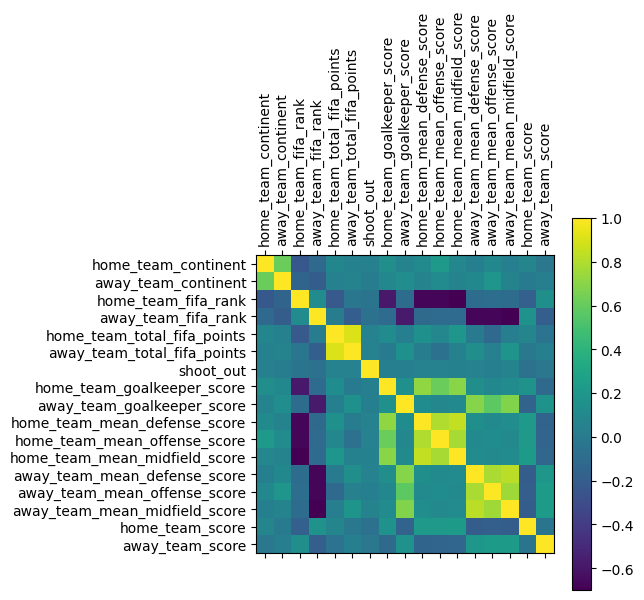
\includegraphics[width=\figsize]{images/correlationMatrix.png}
    \caption{Matriz de correlaciones del conjunto de datos}
    \label{Conjunto-Datos-Matriz-Correlaciones}
\end{figure}

Se puede ver en la figura anterior como no existen relaciones lineales muy destacables en el conjunto de datos y, que en la gran mayoría el valor de correlación se encuentra cercano a cero. Las únicas variables entre las que existe una correlación lineal son las puntuaciones otorgadas por la FIFA en las distintas líneas de juego con la puntuación final del equipo. Después de este breve estudio se ha querido comparar ambas variables objetivas con los datos del conjunto, buscando la existencia de alguna relación lineal. Este estudio se encuentra en las Figuras \ref{Conjunto-Datos-Home-Correlaciones} y \ref{Conjunto-Datos-Away-Correlaciones}.

\begin{figure}[H]
    \centering
    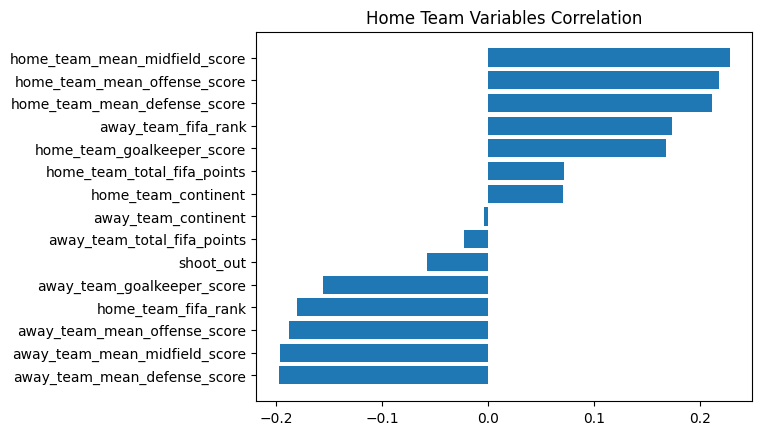
\includegraphics[width=\figsize]{images/homeTeamCorrelation.png}
    \caption{Correlaciones de la variable home\_team\_score}
    \label{Conjunto-Datos-Home-Correlaciones}
\end{figure}

\begin{figure}[H]
    \centering
    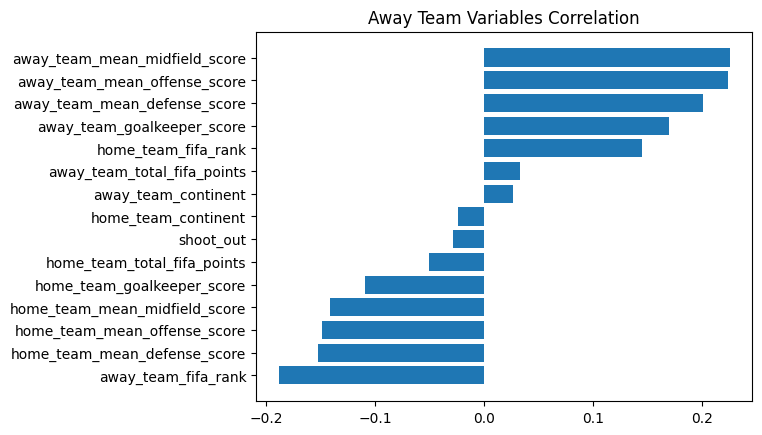
\includegraphics[width=\figsize]{images/awayTeamCorrelation.png}
    \caption{Correlaciones de la variable away\_team\_score}
    \label{Conjunto-Datos-Away-Correlaciones}
\end{figure}

Como se venía comentando en la matriz de correlaciones, no existe ninguna pareja de variables que destaque por una correlación lineal positiva o negativa, y menos que una des estas variables sea del conjunto de variables objetivos. Esto se podría dar por muchos factores, pero, después de muchas horas de tratamiento de los datos, creemos que la componente de aleatoriedad de los datos va a tener más repercusión en los resultados finales de lo esperado.

\subsection{Modificación de la Variable Objetivo}

Con el objetivo de modificar las variancias de las variables objetivo y, intentar adquirir mejores resultados, se ha creído que operar con el valor de la diferencia de las variables objetivos podría ayudar a los modelos a obtener un mejor resultado. Al calcular la variable resultado mediante la resta de las variables home\_team\_score y away\_team\_score, podemos afirmar que un valor positivo en la variable resultado equivale a decir que el equipo local ha salido victorioso del partido, por otra parte, un resultado negativo equivale a la victoria del equipo visitante. Por último, un resultado equivalente a cero, significa empate en el partido. Este estudio ha empezado analizando la matriz de correlación, que se encuentra en la Figura \ref{Conjunto-Datos-Matriz-Correlaciones-Una-Variable}

\begin{figure}[H]
\centering
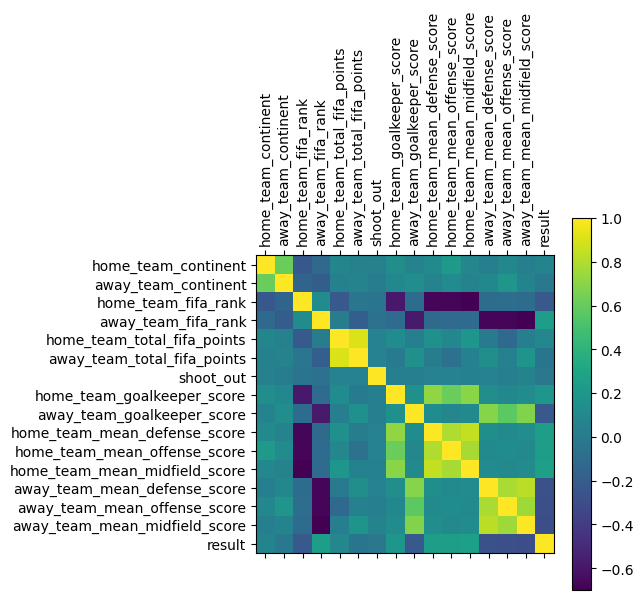
\includegraphics[width=\figsize]{images/correlationMatrixOneObjectiveVariable.png}
\caption{Matriz de correlaciones del conjunto de datos con una variable objetivo}
\label{Conjunto-Datos-Matriz-Correlaciones-Una-Variable}
\end{figure}

Aparentemente, las correlaciones de las variables no se han modificado demasiado, aunque para obtener unos resultados exhaustivos se compararan las Figuras \ref{Conjunto-Datos-Home-Correlaciones}, \ref{Conjunto-Datos-Away-Correlaciones} y \ref{Conjunto-Datos-Resultado-Correlaciones}.

\begin{figure}[H]
\centering
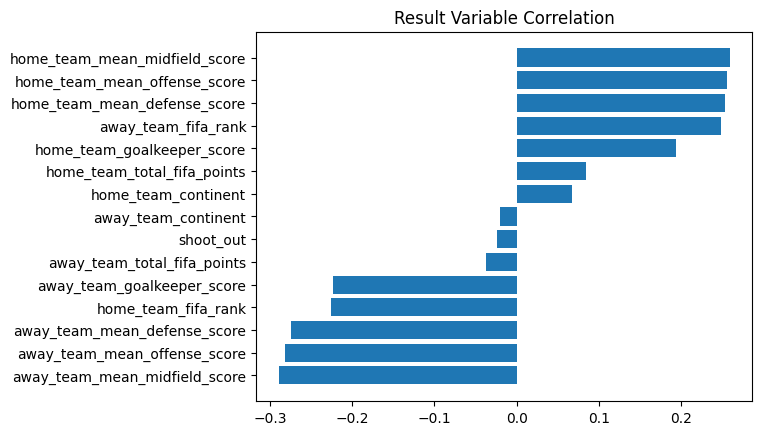
\includegraphics[width=\smallSize]{images/resultCorrelation.png}
\caption{Correlaciones de la variable resultado}
\label{Conjunto-Datos-Resultado-Correlaciones}
\end{figure}

De la gráfica anterior se puede ver la existencia de una correlación positiva entre la variable resultado y todos los datos relacionados con el equipo local. Esta correlación se puede dar a raíz de que una victoria del equipo local equivale a un resultado positivo. Por otra parte, se puede ver como el intervalo de valores de las correlaciones se ha mantenido en relación a las correlaciones del conjunto de datos con dos variables objetivo.
\subsection{Reducción de la dimensionalidad}

Como se ha podido observar, nuestro conjunto de datos no destaca por la existencia de componentes con alta correlación con las variables objetivo, un hecho que dificultará la obtención de resultados destacables. Mediante la reducción de dimensionalidad y el Análisis de Componentes Principales (PCA) se buscará una combinación lineal de las variables originales que capture la mayor cantidad de variabilidad en los datos posible. Esto se logra a través del uso de componentes principales.
\newline

Para no implementar manualmente el Análisis de Componentes Principales se ha optado por usar una funcionalidad de la librería de \cite{Scikit-learn}. Se empezará el estudio con el análisis de los autovalores, también conocidos como eigenvalues. Para realizar el estudio se ha generado la representación gráfica de la cantidad de varianza explicada por cada componente principal. Esta representación, también conocida como Scree Plot se puede visualizar en la Figura \ref{Conjunto-Datos-Scree-Plot}.

\begin{figure}[H]
    \centering
    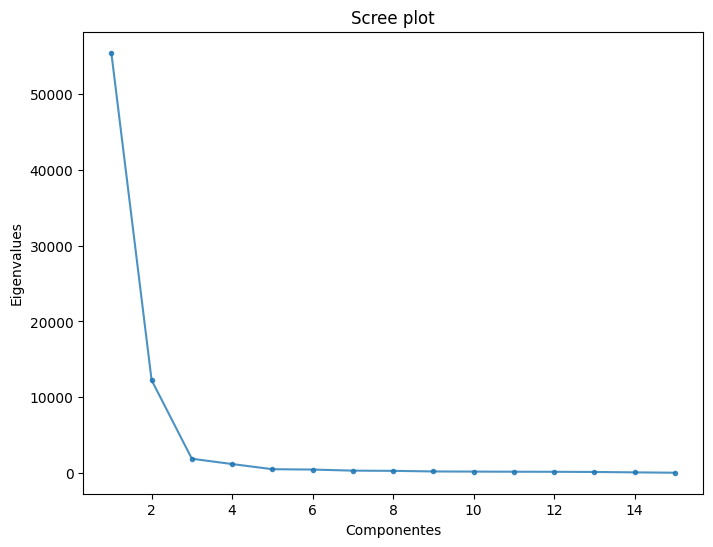
\includegraphics[width=\figsize]{images/screePlot.png}
    \caption{Análisis de Componentes Principales: Scree Plot}
    \label{Conjunto-Datos-Scree-Plot}
\end{figure}

A simple vista se puede evaluar la bondad de ajuste del modelo de PCA. Podemos ver como la mayor parte de la varianza de los datos originales se explica en las primeras componentes, lo que nos permite deducir que el modelo de PCA tiene un buen ajuste. Además, si entramos un poco más en detalle, podemos observar como el número óptimo de componentes principales es 8, ya que en ese punto, encontramos una estabilización de la gráfica, hecho que nos permite afirmar, que usando más de 8 componentes principales estamos perdiendo varianza explicada. Estas conclusiones se han podido comprobar con el gráfico de la Figura \ref{Conjunto-Datos-Varianza-Explicada}. Se puede ver como a partir de la tercera componente, la varianza explicada se mantiene y, por lo tanto, añadir más componentes nos generara ruido en el resultado final.

\begin{figure}[H]
    \centering
    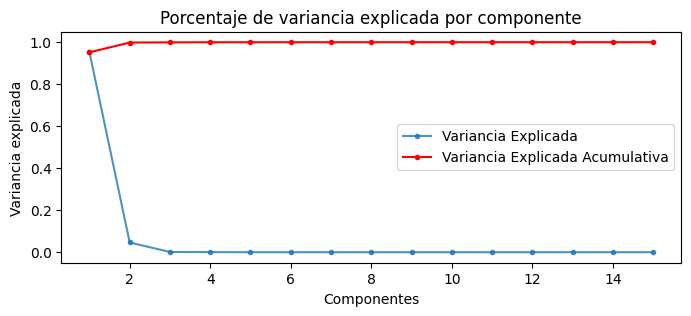
\includegraphics[width=\figsize]{images/varianzaExplicada.png}
    \caption{Análisis de Componentes Principales: Varianza Explicada}
    \label{Conjunto-Datos-Varianza-Explicada}
\end{figure}

El estudio ha finalizado buscando patrones con 2 y 3 componentes. Para realizar el estudio se han generado las Figuras \ref{Conjunto-Datos-Scatter-Plot-2} y \ref{Conjunto-Datos-Scatter-Plot-3}. De ambas visualizaciones podemos sacar las mismas conclusiones, no existen patrones en los datos que nos permitan ajustar fácilmente una recta de regresión, un hecho que va en sintonía con nuestras hipótesis, será altamente complicado obtener resultados satisfactorios debido a la gran variabilidad de los datos.

\begin{figure}[H]
    \centering
    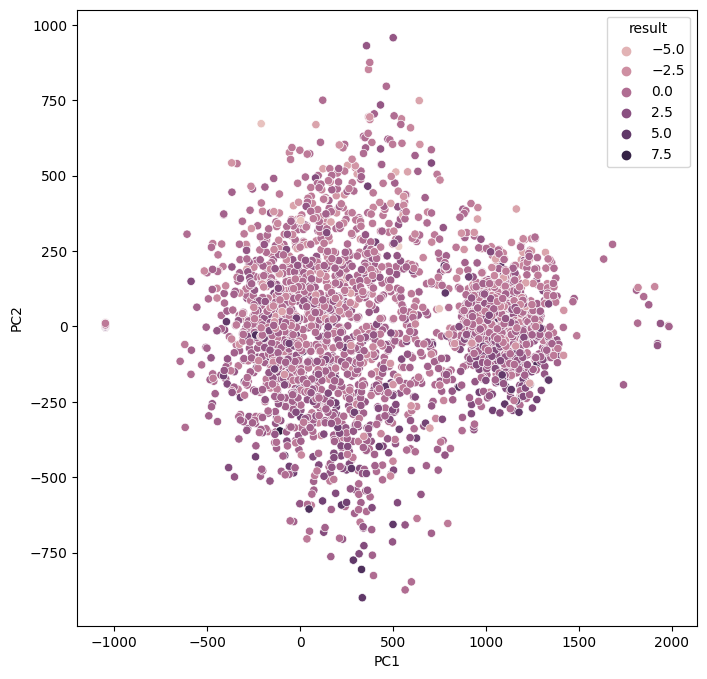
\includegraphics[width=\figsize]{images/scatterPlotPCA2.png}
    \caption{Análisis de Componentes Principales: Dispersión 2 Componentes}
    \label{Conjunto-Datos-Scatter-Plot-2}
\end{figure}

\begin{figure}[H]
    \centering
    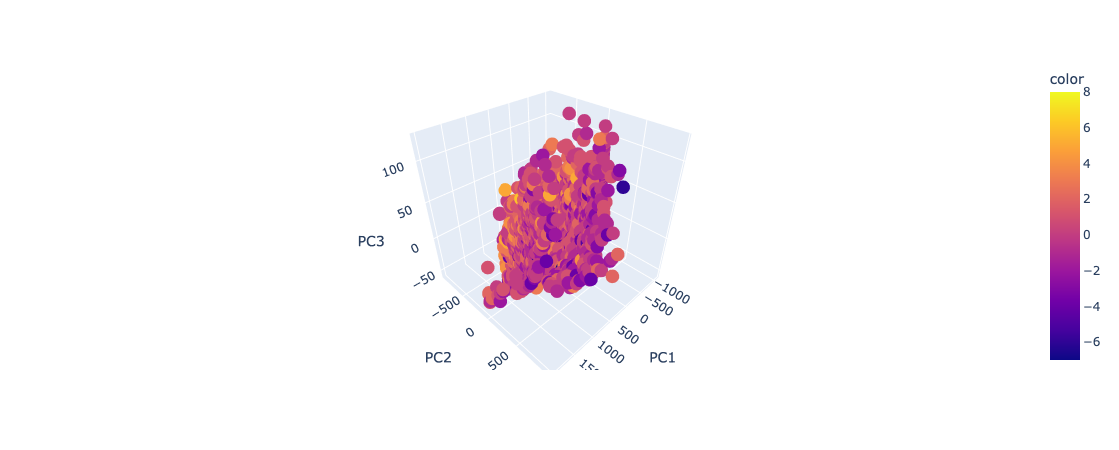
\includegraphics[width=\figsize]{images/scatterPlotPCA3.png}
    \caption{Análisis de Componentes Principales: Dispersión 3 Componentes}
    \label{Conjunto-Datos-Scatter-Plot-3}
\end{figure}

\newpage